\documentclass[11pt, oneside]{article}
\usepackage[letterpaper, margin=2cm]{geometry}
\usepackage{MATH565}

\begin{document}
\noindent \textbf{\Large{Caleb Logemann \\
MATH 565 Continuous Optimization \\
Homework 5
}}

%\lstinputlisting[language=Python]{H01_23.m}
\begin{enumerate}
  \item % #1 Done
    Page 269: Problem 10.1 \\
    Let $J$ be an $m \times n$ matrix $m \ge n$.
    \begin{enumerate}
      \item[(a)] % Done
        Show that $J$ has full column rank if and only if $J^T J$ is nonsingular.

        \begin{proof}
          Suppose that $J$ has full column rank, then $J$ has a full singular
          value decomposition.
          That is $J = U \Sigma V^T$, where $U$ is an orthogonal $m \times m$
          matrix, $V$ is an orthogonal $n \times n$ matrix and $\Sigma$ is a
          diagonal $m \times n$ matrix.
          Since $J$ is full column rank this implies that the diagonal of
          $\Sigma$ is nonzero.
          Now using this decomposition $J^T J$ can be written as
          \[
            J^T J = (U \Sigma V^T)^T (U \Sigma V^T) = V \Sigma^T U^T U \Sigma V^T = V \Sigma^T \Sigma V^T.
          \]
          Note that $\Sigma^T \Sigma$ is a $n \times n$ matrix, and it is
          diagonal as it is the product of diagonal matrices.
          Also the diagonal of $\Sigma^T \Sigma$ is nonzero, as the diagonal of
          $\Sigma$ is nonzero.
          Thus this shows that $J^T J$ can be diagonalized as
          $V \Sigma^T \Sigma V^T$ and that the eigenvalues are nonzero.
          Therefore $J^T J$ is nonsingular as the eigenvalues are nonzero.

          Now suppose that $J^T J$ is nonsingular.
          If $J$ has full column rank, then the equation $Jx = 0$ will only
          have the trivial solution.
          Suppose to the contrary that there exists $x \in \RR^n$ such that
          $Jx = 0$ and $x \neq 0$.
          Multiplying both sides of this equation $J^T$ we see that this
          indicates that $J^T J x = 0$.
          However $J^T J$ is nonsingular and so is invertible, which implies
          that
          \[
            x = (J^T J)^{-1} 0 = 0.
          \]
          This is a contradiction, therefore $J$ must have full column rank.
        \end{proof}

      \item[(b)] % Done
        Show that $J$ has full column rank if and only if $J^T J$ is positive definite.

        \begin{proof}
          Suppose that $J^T J$ is positive definite.
          This implies that the eigenvalues of $J^T J$ are all strictly greater
          than zero.
          Since all of the eigenvalues are strictly positive, this implies that
          $\det(J^T J) > 0$ or equivalently that $J^T J$ is nonsingular.
          Now by part (a) this implies that $J$ has full column rank.

          Suppose on the other hand $J$ has full column rank.
          Now by part (a) this implies that $J^T J$ is nonsingular.
          Since $J^T J$ is nonsingular, the eigenvalues of $J^T J$ are nonzero.
          As in part (a) it was shown that $J^T J$ could be diagonalized as
          $V \Sigma^T \Sigma V^T$.
          Considering the diagonal of $\Sigma^T \Sigma$, we see that the
          eigenvalues of $J^T J$ are the squares of the singular values of $J$.
          Since squares are all nonnegative, this shows that the eigenvalues
          of $J^T J$ are nonnegative.
          This fact along with the fact that the eigenvalues are nonzero implies
          that $J^T J$ has only positive eigenvalues or equivalently that $J^T J$
          is positive definite.
        \end{proof}
    \end{enumerate}

  \item % #2 Done
    Page 269: Problem 10.5 \\
    Suppose that each residual function $r_j$ and its gradient are Lipschitz
    continuous with Lipschitz constant L, that is,
    \[
      \abs{r_j(x) - r_j(x^*)} \le L \norm{x - x^*}, \quad \norm{\nabla r_j(x) - \nabla r_j(x^*)} \le L \norm{x - x^*}
    \]
    for all $j = 1, 2, \ldots, m$ and all $x, x^* \in D$, where $D$ is a
    compact subset of $\RR^n$.
    Assume also that the $r_j$ are bounded on $D$, that is, there exists $M > 0$
    such that $\abs{r_j(x)} \le M$ for all $j = 1, 2, \ldots, m$ and all
    $x \in D$.
    Find Lipschitz constants for the Jacobian $J$ (10.3) and the gradient
    $\nabla f$ (10.4) over $D$.

    First I will suppose that all norms are the 2-norm or the matrix norm
    induced by the vector 2-norm.
    First I will consider the Jacobian.
    \begin{align*}
      \norm{J(x) - J(x^*)} &= \sup[\norm{y} = 1]{\norm{(J(x) - J(x^*))y}} \\
      &= \sup[\norm{y} = 1]{\sqrt{\sum*{j = 1}{m}{\p{(\nabla r_j(x) - \nabla r_j(x^*))^T y}^2}}}
      \intertext{Using the Cauchy-Schwarz inequality}
      &\le \sup[\norm{y} = 1]{\sqrt{\sum*{j = 1}{m}{\p{\norm{\nabla r_j(x) - \nabla r_j(x^*)} \norm{y}}^2}}} \\
      &= \sqrt{\sum*{j = 1}{m}{\norm{\nabla r_j(x) - \nabla r_j(x^*)}^2}}
      \intertext{Using the Lipschitz continuity of the gradient}
      &\le \sqrt{\sum*{j = 1}{m}{L^2\norm{x - x^*}^2}} \\
      &= \sqrt{mL^2\norm{x - x^*}^2} \\
      &= \sqrt{m}L\norm{x - x^*} \\
    \end{align*}
    Therefore a Lipschitz constant for the Jacobian is $\sqrt{m}L$.

    Now I will consider the gradient $\nabla f$.
    \begin{align*}
      \norm{\nabla f(x) - \nabla f(x^*)} &= \norm{J(x)^T r(x) - J(x^*)^T r(x^*)} \\
      &= \norm{J(x)^T r(x) - J(x^*)^T r(x) + J(x^*)^T r(x) - J(x^*)^T r(x^*)} \\
      &= \norm{(J(x) - J(x^*))^T r(x) + J(x^*)^T (r(x) - r(x^*))} \\
      &\le \norm{(J(x) - J(x^*))^T r(x)} + \norm{J(x^*)^T (r(x) - r(x^*))} \\
      &\le \norm{J(x) - J(x^*)} \norm{r(x)} + \norm{J(x^*)} \norm{r(x) - r(x^*)} \\
      &\le \sqrt{m}L \norm{x - x^*} \norm{r(x)} + L \norm{J(x^*)} \norm{x - x^*}
    \end{align*}
    Since $r_j$ is bounded on a compact set $D$, $\norm{r(x)}$ achieves
    its maximum on $D$.
    Let $A = \max[x \in D]{\norm{r(x)}}$.
    Also we have shown that the Jacobian is bounded and Lipschitz
    continuous on the compact set $D$, so there exists
    $B = \max[x \in D]{\norm{J(x)}}$.
    Now we can see that
    \begin{align*}
      \norm{\nabla f(x) - \nabla f(x^*)} &\le \sqrt{m}L A\norm{x - x^*} + L B \norm{x - x^*} \\
      &= \p{\sqrt{m} A + B} L \norm{x - x^*}
    \end{align*}
    This shows that the Lipschitz constant for $\nabla f$ is
    $\p{\sqrt{m} A + B} L$.

  \item % #3 Done
    Consider the underdetermined linear system $Jx = r$, where
    $J \in \RR^{m \times n}$, $x \in \RR^n$, $r \in \RR^m$, and $m < n$
    (i.e. there are less equations than unknowns).
    Assume that the rank of $J$ is $m$ (i.e., it has full rank).
    There will exist infinitely many solutions.
    The minimum norm solution of $Jx = r$ is the solution closest to the origin,
    which may be regarded as the solution of the constrained optimization problem:
    \[
      \min*[x \in \RR^n]{\norm{x}^2} \quad \text{subject to} \quad Jx = r.
    \]
    \begin{enumerate}
      \item[(a)]
        Use the Lagrange multiplier method, derive the solution to this
        optimization problem:
        \[
          x = J^T (J J^T)^{-1} r
        \]

        \begin{proof}
          The Lagrange multiplier method states that the solution to this
          minimization problem satisfies the following equations,
          \begin{align*}
            \nabla_x \mcL(x, \lambda) &= 0, \\
            c_i(x) &= 0, \forall i \in \mcE, \\
            c_i(x) &\ge 0, \forall i \in \mcI, \\
            \lambda_i &\ge, \forall i \in \mcI, \\
            \lambda_i c_i(x) &= 0, \forall i \in \mcE \cup \mcI,
          \end{align*}
          where $\mcL$ is the Lagrangian.
          In this problem the Lagrangian is
          \[
            \mcL(x, \lambda) = \norm{x}^2 - \lambda^T (Jx - r).
          \]
          There are only equality constraints which are
          \[
            Jx - r = 0
          \]
          The full set of equations for this problem is thus
          \begin{align*}
            \nabla_x (\norm{x}^2 - \lambda^T (Jx - r)) &= 0, \\
            Jx - r &= 0, \\
            \lambda^T (Jx - r) &= 0,
          \end{align*}
          The last equation is redundant with the second equation, so only the
          first two equations are necessary.
          Evaluating the gradient in the first equation gives
          \[
            2x - J^T \lambda = 0
          \]
          Solving this for $x$ gives
          \[
            x = \frac{1}{2} J^T \lambda
          \]
          Substituting this into the second equation and solving for $\lambda$
          gives
          \begin{align*}
            Jx - r &= 0 \\
            \frac{1}{2} J J^T \lambda - r &= 0 \\
            J J^T \lambda &= 2 r.
            \intertext{Now since $J$ has full rank the matrix $J J^T$ is
            invertible, which gives}
            \lambda &= 2(J J^T)^{-1} r
          \end{align*}
          Now we can find $x$ to be
          \[
            x = J^T (J J^T)^{-1} r
          \]
          as necessary.
        \end{proof}

      \item[(b)]
        Find the minimum norm solution of the $3 \times 5$ system $Jx = r$,
        where
        \[
          J =
          \begin{pmatrix}
            1 & 2 & 0 & 3 & 2 \\
            -1 & -1 & 4 & 2 & 0 \\
            3 & -2 & 2 & 1 & 1
          \end{pmatrix},
          \quad
          r =
          \begin{pmatrix}
            4 \\
            1 \\
            -7
          \end{pmatrix}.
        \]

        Using part (a) we see that
        \[
          x = J^T (J J^T)^{-1} r
        \]
        is the minimum norm solution.
        This can be found using \MATLAB to be
        \[
          x =
          \begin{bmatrix}
            -1.5362 \\
            1.4624 \\
            -0.1802 \\
            0.8236 \\
            0.0703
          \end{bmatrix}
        \]
    \end{enumerate}

  \item % #4 Done
    An important problem in signal processing amounts to finding parameters
    $c_1, c_2, \ldots, c_n$ and $\lambda_1, \lambda_2, \ldots, \lambda_n$ such
    that
    \[
      \sum{k=1}{n}{c_k e^{-\lambda_k t}} \approx f(t),
    \]
    for a given signal function $f(t)$.
    One approach for solving this problem is to formulate a nonlinear least
    squares problems.
    Let
    \[
      x := (x_1, x_2, \ldots, x_{2n}) = (c_1, \ldots, c_n, \lambda_1, \ldots, \lambda_n)
    \]
    be the vector of parameters to be determined.
    Let $s_j = f(t_j)$ be given samples of $f$ for $j = 1,\ldots,2n$ and set
    \[
      r_j(x) = \sum{k=1}{n}{c_k e^{-\lambda_k t_j}} - s_j = \sum{k=1}{n}{x_k e^{-x_{n+k}t_j}} - s_j.
    \]
    We then obtain the parameters as the solution of the nonlinear least squares
    problem:
    \[
      \min*[x \in \RR^{2n}]{\norm{r(x)}^2}.
    \]
    \begin{enumerate}
      \item[(a)]
        Find the general expression for $J(x)$.

        The i, j entry of the Jacobian is defined as
        \[
          J(x)_{ij} = \pd{r_j}{x_i}
        \]
        This value can be computed using the following definition of $r_j$ for
        this problem,
        \[
          r_j(x) = \sum{k=1}{n}{c_k e^{-\lambda_k t_j}} - s_j = \sum{k=1}{n}{x_k e^{-x_{n+k}t_j}} - s_j.
        \]
        The entries are
        \begin{align*}
          J(x)_{ij} &= \pd{r_j}{x_i} \\
          &= \pda{\sum{k=1}{n}{x_k e^{-x_{n+k}t_j}} - s_j}{x_i}
          \intertext{If $i \le n$, then there exists $k = i$, so}
          J(x)_{ij} &= e^{-x_{n+i}t_j}
          \intertext{If $i > n$, then there exists $k$ such that $i = n+k$, so}
          J(x)_{ij} &= -t_j x_{i-n} e^{-x_i t_j}
        \end{align*}
        Thus the general definition of the Jacobian by entry is
        \[
          J(x)_{ij} =
          \begin{cases}
            e^{-x_{n+i}t_j} & i \le n \\
            -t_j x_{i-n} e^{-x_i t_j} & i > n
          \end{cases}
        \]
        where $i, j = 1, 2, \ldots, 2n$.

      \item[(b)]
        Let $n = 2$, and
        \[
          t = (0.0, 0.3, 0.6, 0.9) \quad \text{and} \quad s = (2.700, 1.480, 0.819, 0.458).
        \]
        In \MATLAB or \PYTHON, program a Gauss-Newton iteration scheme for this
        problem.
        Apply the scheme the following initial guess:
        \[
          x_0 = (1, 1, 1, 2)
        \]
        and run until convergence.

        The following function implements the Gauss-Newton iteration with an
        constant step of $\alpha = 1$.
        \lstinputlisting[language=Matlab]{gaussNewton.m}
        The following script uses the previous function to solve the given
        nonlinear least squares problem.
        This script uses a tolerance of $10^{-10}$ and a maximum of a 1000
        iterations.
        \lstinputlisting[language=Matlab]{H05_4.m}
        The Gauss-Newton converges in 8 steps to the solution
        $(0.5756, 2.1244, 1.4307, 2.1780)$, that is $c_1 = 0.5756$, $c_2 = 2.1244$,
        $\lambda_1 = 1.4307$, and $\lambda_2 = 2.1780$.
        The following plot is also produced which verfies that these are
        indeed the correct values.
        \begin{center}
          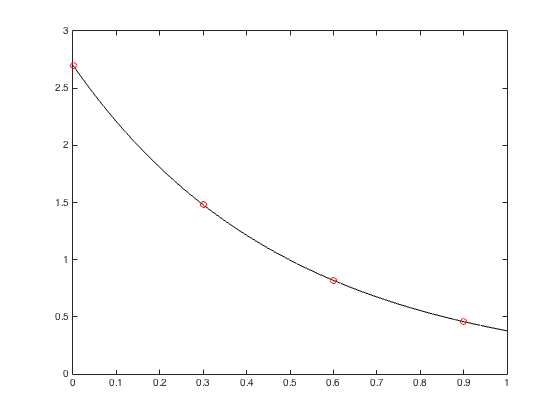
\includegraphics[scale=.5]{Figures/05_1}
        \end{center}
    \end{enumerate}

  \item % #5 Done
    Page 352: Problem 12.4 \\
    If $f$ is convex and the feasible region $\Omega$ is convex, show that local
    solutions of the problem (12.3) are also global solutions.
    Show that the set of global solutions is convex.
    (Hint: See Theorem 2.5.)

    \begin{proof}
      Let $f$ be a convex function and let $\Omega$, the feasible region, be
      convex.
      Suppose that $x$ is a local minimum of $f$, but not a global minimum
      This implies that there exists $x^* \Omega$, a global minimum, such that
      $f(x^*) < f(x)$.
      Since $\Omega$ is convex this implies that $tx + (1-t)x^* \in \Omega$
      for all $t \in \br{0, 1}$.
      Also since $f$ is convex,
      \begin{align*}
        f(tx + (1-t)x^*) &\le tf(x) + (1-t)f(x^*) \\
        &\le tf(x) + (1-t)f(x) \\
        &= f(x)
      \end{align*}
      Now for any local neighborhood, $N$, of $x$, there exists a
      $t \in \br{0, 1}$ such that $tx + (1-t)x^* \in N$ and
      $f(tx + (1-t)x^*) < f(x)$.
      This directly contradicts the fact that $x$ is a local minumum, therefore
      if $x$ is a local minimum it must also be a global minimum.
    \end{proof}

  \item % #6 Done
    Page 353: Problem 12.13 \\
    Show that for the feasible region defined by
    \begin{align*}
      (x_1 - 1)^2 + (x_2 - 1)^2 \le 2, \\
      (x_1 - 1)^2 + (x_2 + 1)^2 \le 2, \\
      x_1 \ge 0,
    \end{align*}
    the MFCG is satisfied at $x^* = (0, 0)^T$ but the LICQ is not satisfied.

    \begin{proof}
      First note that $\set{\nabla c_i(x^*), i \in \mcE}$ is empty as there are
      no equality constraints.
      Therefore this set is trivially linearly independent.

      Second the MFCQ require the the gradients of the constraints by computed.
      Let
      \begin{align*}
        c_1(x) &= 2 - (x_1-1)^2 - (x_2-1)^2 \\
        c_2(x) &= 2 - (x_1-1)^2 - (x_2+1)^2 \\
        c_3(x) &= x_1
      \end{align*}
      where $\mcI = \set{1, 2, 3}$ and $\mcE = \varnothing$.
      Then the gradients of the constraints are
      \begin{align*}
        \nabla c_1(x) &=
        \begin{bmatrix}
          -2(x_1 - 1) \\
          -2(x_2 - 1)
        \end{bmatrix} \\
        \nabla c_2(x) &=
        \begin{bmatrix}
          -2(x_1 - 1) \\
          -2(x_2 + 1)
        \end{bmatrix} \\
        \nabla c_3(x) &=
        \begin{bmatrix}
          1 \\
          0
        \end{bmatrix}.
      \end{align*}
      At the point $x^* = (0, 0)$, these gradients are
      \begin{align*}
        \nabla c_1(x^*) &=
        \begin{bmatrix}
          2 \\
          2 
        \end{bmatrix} \\
        \nabla c_2(x^*) &=
        \begin{bmatrix}
          2 \\
          -2
        \end{bmatrix} \\
        \nabla c_3(x^*) &=
        \begin{bmatrix}
          1 \\
          0
        \end{bmatrix}.
      \end{align*}


      At the point $x^* = (0, 0)$, all of the inequality constraints are active.
      Consider the vector $w = \br{1, 0}^T$, then
      \begin{align*}
        \nabla c_1(x^*)^T w &=
        \begin{bmatrix}
          2 & 2
        \end{bmatrix}
        \begin{bmatrix}
          1 \\
          0
        \end{bmatrix} \\
        &= 2 > 0 \\
        \nabla c_2(x^*)^T w &=
        \begin{bmatrix}
          2 & -2
        \end{bmatrix}
        \begin{bmatrix}
          1 \\
          0
        \end{bmatrix} \\
        &= 2 > 0 \\
        \nabla c_3(x^*)^T w &=
        \begin{bmatrix}
          1 & 0
        \end{bmatrix}
        \begin{bmatrix}
          1 \\
          0
        \end{bmatrix} \\
        &= 1 > 0
      \end{align*}
      This shows that these constraints satisfy the MFCQ is satisfied at $x^* = \br{0, 0}^T$.

      Now consider the LICQ, the vectors
      $\set{\nabla c_i(x^*): i \in \mcA(x^*) \cap \mcI}$ are not linearly
      independent as the set contains 3 vectors in $\RR^2$.
    \end{proof}

  \item % #7 Done
    Page 354: Problem 12.18 \\
    Consider the problem of finding the point on the parabola
    $y = \frac{1}{5}(x - 1)^2$ that is closest to $(x, y) = (1, 2)$, in the
    Euclidean norm sense.
    We can formulate this problem as
    \[
      \min*{f(x, y)} = (x - 1)^2 + (y - 2)^2 \quad \text{subject to } (x - 1)^2 = 5y.
    \]
    \begin{enumerate}
      \item[(a)] % Done
        Find all the KKT points for this problem.
        Is the LICQ satisfied?

        For this problem the Lagrangian is
        \[
          \mcL(x, y, \lambda) = (x - 1)^2 + (y - 2)^2 - \lambda\p{(x - 1)^2 - 5y}.
        \]
        The gradient of the Lagrangian is then
        \[
          \nabla_{x,y} \mcL(x, y, \lambda) =
          \begin{bmatrix}
            (2 - 2\lambda)(x - 1) \\
            2(y - 2) + 5\lambda
          \end{bmatrix}
        \]

        The KKT conditions are thus
        \begin{align*}
          (2 - 2\lambda)(x - 1) &= 0 \\
          2(y - 2) + 5\lambda &= 0 \\
          (x - 1)^2 - 5y &= 0 \\
          \lambda((x - 1)^2 - 5y) &= 0
        \end{align*}
        The last equation is redundant with the third equation.
        The first three equations can be solved as follows.
        \begin{align*}
          y &= \frac{1}{5}(x - 1)^2 \\
          0 &= 2(y - 2) + 5\lambda \\
          0 &= 2\p{\frac{1}{5}(x - 1)^2 - 2} + 5\lambda \\
          -5\lambda &= \frac{2}{5}(x - 1)^2 - 4 \\
          \lambda &= -\frac{2}{25}(x - 1)^2 + \frac{4}{5} \\
          0 &= (2 - 2\lambda)(x - 1) \\
          0 &= (2 + \frac{4}{25}(x - 1)^2 - \frac{8}{5})(x - 1) \\
          0 &= (\frac{4}{25}(x - 1)^2 + \frac{2}{5})(x - 1)
          \intertext{either}
          x &= 1
          \intertext{or}
          0 &= \frac{4}{25}(x - 1)^2 + \frac{2}{5} \\
          -\frac{2}{5} &= -\frac{4}{25}(x - 1)^2 \\
          -\frac{2}{5} \frac{25}{4} &= (x - 1)^2 \\
          -\frac{5}{2} &= (x - 1)^2 \\
          \pm\sqrt{-\frac{5}{2}} &= x - 1 \\
          x &= 1 \pm i\sqrt{\frac{5}{2}} \\
        \end{align*}
        There are three points which satisfy the KKT conditions.
        The first is at $x = 1$, and in this case $y = 0$ and
        $\lambda = -\frac{4}{5}$.
        The second is at $x = 1 + i\sqrt{\frac{5}{2}}$, and in this case $y = -\frac{1}{2}$ and
        $\lambda = 1$.
        The third point is $x = 1 - i\sqrt{\frac{5}{2}}$, and in this case $y = -\frac{1}{2}$ and
        $\lambda = 1$.

        In order to see if any of these points satisfy the LICQ, the gradients
        of the active constraints must be computed.
        Since there is only one constraint and it is active for all points
        satsifying the KKT conditions, the set containing this vector is
        linearly independent.
        Note that this gradient is nonzero at this point as the $y$ derivative
        is $-5$.

      \item[(b)] % Done
        Which of these points are the solutions?

        Plugging these points into the objective function allows us to find the
        solutions to the minimization problem.
        At the point $(x, y) = (1, 0)$, the objective function is $f(1, 0) = 16$.
        At the points $(1 + i\sqrt{\frac{5}{2}}, -\frac{1}{2})$ and $(1 - i\sqrt{\frac{5}{2}}, -\frac{1}{2})$ the
        objective function is $f = 3.75$.
        However since the second and third points are not real valued, the
        solution is the point $(x, y) = (1, 0)$.

      \item[(c)] % Done
        By directly substituting the constraint into the object function and
        eliminating the variable $x$, we obtain an unconstrained optimization
        problem.
        Show that the solutions of this problem cannot be solutions of the
        original problem.

        In order to substitute and elimination the variable $x$ we need to first
        solve the constraint for $x$.
        \begin{align*}
          (x - 1)^2 &= 5y \\
          x - 1 &= \pm\sqrt{5y} \\
          x &= \pm\sqrt{5y} + 1 \\
        \end{align*}
        Thus the problem can now be expressed as
        \[
          \min[y \in \RR]{(\pm\sqrt{5y} + 1 - 1)^2 + (y - 2)^2}
        \]
        This minimum can be found using basic calculus techniques.
        \begin{align*}
          f(y) &= (\pm\sqrt{5y} + 1 - 1)^2 + (y - 2)^2 \\
          &= 5y + (y - 2)^2 \\
          &= y^2 + y - 4 \\
          f'(y) &= 2y + 1 \\
          f'(y) &= 0 \\
          y &= -\frac{1}{2} \\
          f''(y) &= 2
        \end{align*}
        This shows that the minimum of $f$ is at $y = -\frac{1}{2}$.
        This is in fact a minumum as $f''(-\frac{1}{2}) > 0$.

        This can't be a solution because at $y = -1/2$, then
        $x = 1 \pm i \sqrt{\frac{5}{2}}$ which is not real valued.
        These are in fact the two invalid solutions to the constrained problem.
    \end{enumerate}

  \item % #8 Done
    Page 354: Problem 12.21 \\
    Find the maxima of $f(x) = x_1 x_2$ over the unit disk defined by the
    inequality constraint $1 - x_1^2 - x_2^2 \ge 0$.

    This problem can be written as the following minimization problem.
    \[
      \min{-x_1 x_2} \text{ subject to } 1 - x_1^2 - x_2^2 \ge 0
    \]

    The Lagrangian for this problem is thus
    \[
      \mcL(x_1, x_2, \lambda) = -x_1 x_2 - \lambda (1 - x_1^2 - x_2^2).
    \]
    The KKT conditions are now
    \begin{align*}
      -x_2 + 2\lambda x_1 &= 0 \\
      -x_1 + 2\lambda x_2 &= 0 \\
      1 - x_1^2 - x_2^2 &\ge 0 \\
      \lambda &\ge 0 \\
      \lambda (1 - x_1^2 - x_2^2) &= 0
    \end{align*}
    These can be solved as follows.
    \begin{align*}
      0 &= -x_2 + 2\lambda x_1 \\
      x_2 &= 2\lambda x_1 \\
      0 &= -x_1 + 2\lambda x_2 \\
      0 &= -x_1 + 2\lambda (2\lambda x_1) \\
      0 &= -x_1 + 4\lambda^2 x_1 \\
      0 &= (4\lambda^2 - 1) x_1 \\
    \end{align*}
    This shows that either $x_1 = 0$ or $4\lambda^2 - 1 = 0$, which can be
    simplified as
    \begin{align*}
      0 &= 4\lambda^2 - 1 \\
      1 &= 4\lambda^2 \\
      \frac{1}{4} &= \lambda^2 \\
      \lambda &= \pm \frac{1}{2}
    \end{align*}
    Since $\lambda \ge 0$ this implies that $\lambda = \frac{1}{2}$, and also
    that $x_2 = x_1$
    Now since $\lambda \neq 0$, the last KKT condition implies that
    \begin{align*}
      0 &= 1 - x_1^2 - x_2^2 \\
      0 &= 1 - x_1^2 - x_1^2 \\
      0 &= 1 - 2x_1^2 \\
      2x_1^2 &= 1 \\
      x_1 &= \pm \frac{1}{\sqrt{2}} = \pm \frac{\sqrt{2}}{2} \\
    \end{align*}
    Thus the two solutions that satisfy the KKT conditions are
    $\p{\frac{\sqrt{2}}{2}, \frac{\sqrt{2}}{2}}$ and
    $\p{-\frac{\sqrt{2}}{2}, -\frac{\sqrt{2}}{2}}$, with
    $\lambda = \frac{1}{2}$.

    Plugging these points in the objective function we see that
    $-x_1 x_2 = -\frac{1}{2}$ for both points.
    This shows that points of these points are minimzers of $-x_1 x_2$ and thus
    are maximizers of $x_1 x_2$.
\end{enumerate}
\end{document}
